\clearpage
\section*{\currfilename}

\begin{figure}[H]
  \fontsize{10pt}{10pt}\selectfont
  \begin{center}
    \begin{tikzpicture}[auto, scale=0.85, every node/.style={transform shape}, node distance=1.0cm, >=latex']
      \node[squareblock, minimum height=1cm, minimum width=2cm] (block1){Baseline};
      \node[squareblock, below of=block1, node distance=1.5cm, minimum height=1cm, minimum width=2cm] (block2){Adaptive};
      \matrix[ampersand replacement=\&, row sep=0.5cm, left of=block1,node distance=1cm] (block1in) {
        \node [coordinate] (b1inA) {}; \\
        \node [coordinate] (b1inB) {}; \\
      };
      \matrix[ampersand replacement=\&, row sep=0.5cm, left of=block2,node distance=1cm] (block2in) {
        \node [coordinate] (b2inA) {}; \\
        \node [coordinate] (b2inB) {}; \\
      };
      \node [left of=b2inB, node distance=0.5cm] (2B) {};
      \node [below of=2B, node distance=0.12cm] (2B2) {};
      \node [left of=b2inA, node distance=1.0cm] (2A) {};
      \node [below of=2A, node distance=0.12cm] (2A2) {};

      \node[whitesum,right of=block1, node distance=2.0cm] (sum1) {};
      \node[squareblock, minimum height=1cm, minimum width=1.0cm, label=below:{delay}, right of=sum1,node distance=1.5cm] (block3) {$\tau$};
      \node[squareblock, minimum height=1cm, minimum width=1.0cm, label=below:{\shortstack[c]{Actuator\\Dynamics}}, right of=block3,node distance=2.5cm, inner sep= 1mm] (block4) {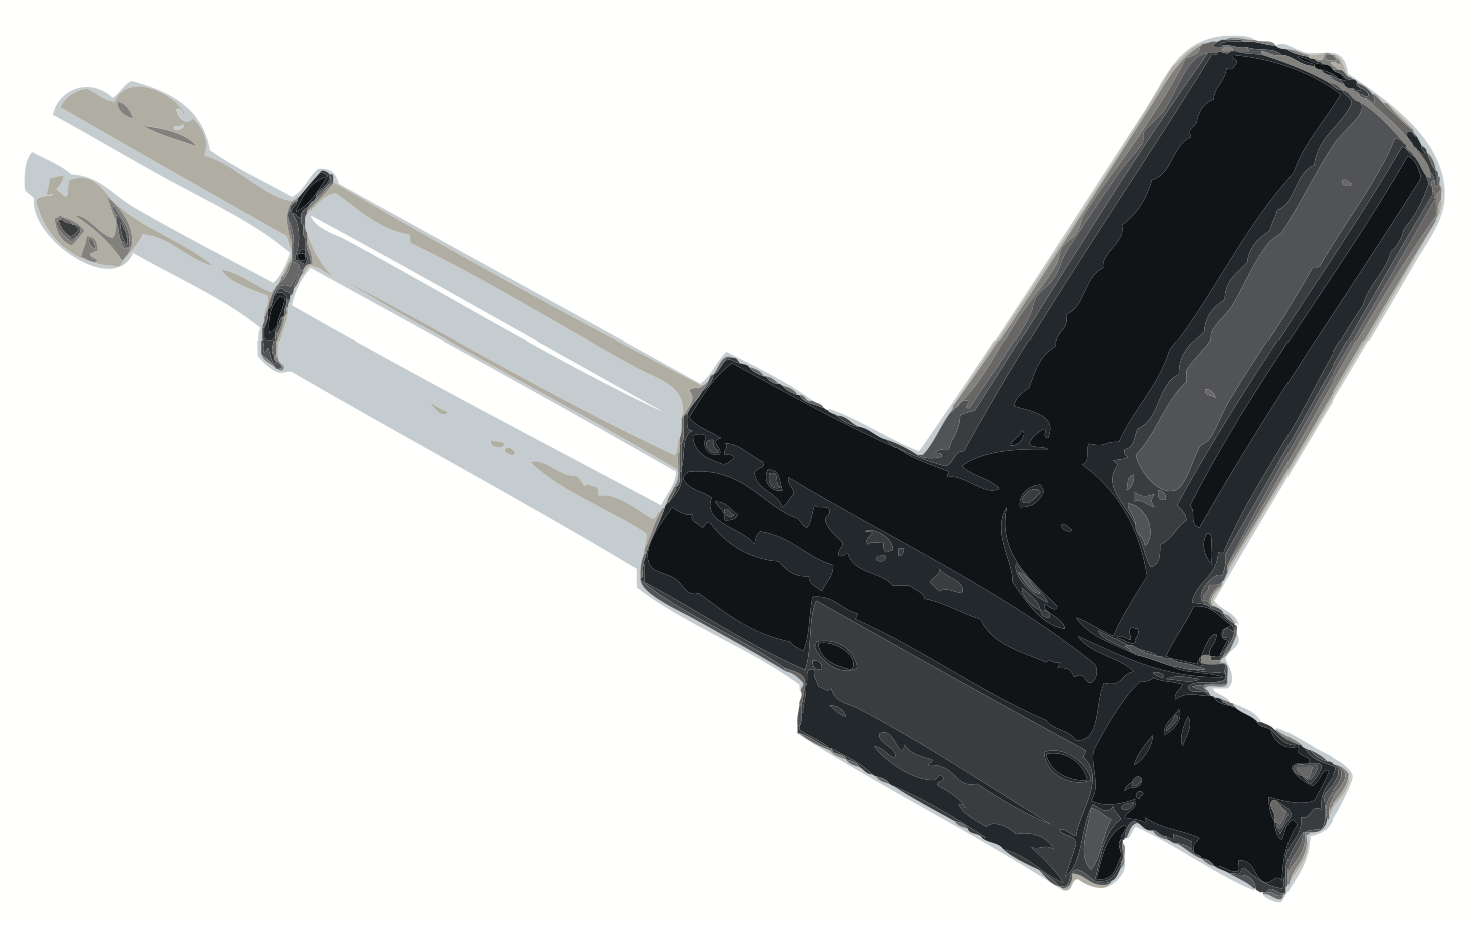
\includegraphics[width=1.6cm]{../fig/actuator_image.png}};
      \node [right of=block4,draw=black, anchor=west,node distance=2.0cm, label=below:{\shortstack[c]{Equations of\\Motion}}, minimum width=2cm, inner sep= 0mm] (block5) {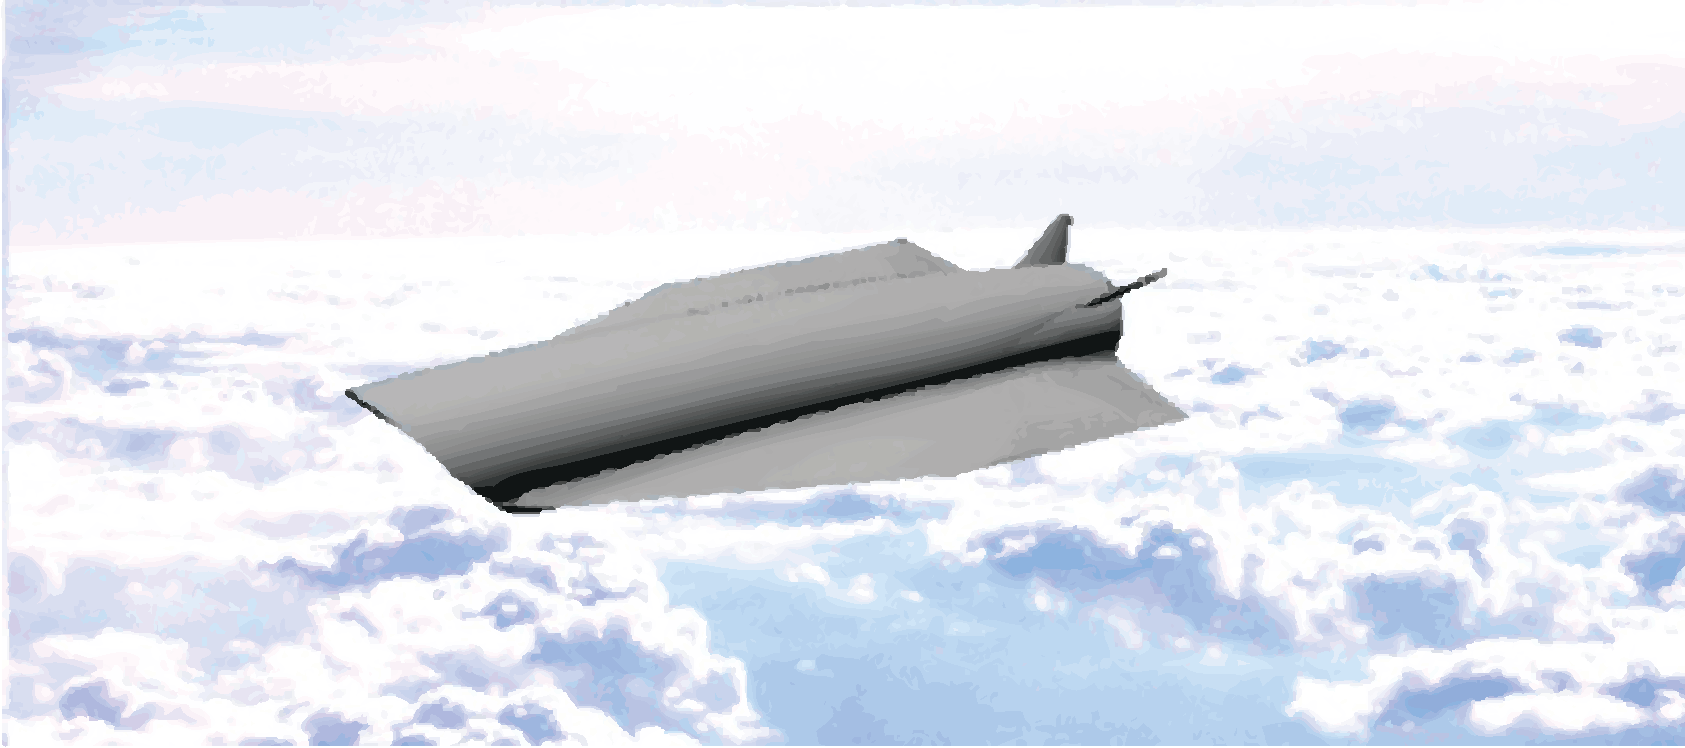
\includegraphics[width=4cm]{../fig/ghvclouds.pdf}};
      \node[whitesum,right of=block5, node distance=3.0cm] (sum2) {};
      \node[squareblock, minimum height=1cm, minimum width=1.0cm, right of=sum2,node distance=1.5cm] (block6) {ZOH};
      \node[squareblock, minimum height=1cm, minimum width=1.0cm, right of=block6,node distance=1.6cm] (block7) {Filter};
      \node[output, right of=block7,node distance=1.5cm] (output1) {};
      \node[input, below of=block2,node distance=1.0cm](input2){};
      \node[input, above of=sum2,node distance=1.0cm](input3){};
      \draw [->] (b1inA) + (-2.5cm,0cm) -> node [pos=0.15]{$z_{\text{cmd}}$}  (b1inA);
      \draw [->] (b1inB) + (-0.5cm,0cm) -> (b1inB);
      \draw [->] (b2inA) + (-1cm,0cm) -> (b2inA);
      \draw [->] (b2inB) + (-2.0cm,0cm) -> node[name=TB,node distance=2.5cm]{} (b2inB);
      \draw[->](block7) --  node[name=yi,pos=0.4]{} (output1);
      \draw[-](yi) |- (input2);
      \draw[-](b1inB) + (-0.5cm,0cm) -- (2B2);
      \draw[-](b1inA) + (-1.0cm,0cm) -- (2A2) ;
      \draw[-] (b2inB) + (-2.0cm,0cm) |- (input2);
      \draw[->](block1) -- (sum1);
      \draw[->](block2) -| (sum1);
      \draw[->](sum1) -- (block3);
      \draw[->](block3) -- (block4);
      \draw[->](block4) -- (block5);
      \draw[->](block5) -- (sum2);
      \draw[->](sum2) -- (block6);
      \draw[->](block6) -- node[name=azoh,pos=0.4]{} (block7);
      \draw[->](input3) -- (sum2);

      \begin{pgfonlayer}{background}
        \path (block1 |- block1)+(-2.5,0.7) node (c) {};
        \path (block2 -| block2)+(2.5,-0.7) node (d) {};
        \path[fill=gray!20, draw, dashed] (c) rectangle (d);
      \end{pgfonlayer}

      \begin{pgfonlayer}{background}
        \path (block6 |- block6)+(-0.7,0.7) node (c) {};
        \path (block7 -| block7)+(0.7,-0.7) node (d) {};
        \path[fill=gray!20, draw, dashed] (c) rectangle (d);
      \end{pgfonlayer}

      % \node [below of=block2, node distance = 0.9cm] {Controller};
      \node [above of=block1, node distance = 0.9cm] {100 Hz};
      \node [above of=azoh, node distance = 0.8cm] {600 Hz};
      \node [above of=sum2, node distance = 1.2cm] {noise};
    \end{tikzpicture}
    \caption{Baseline plus adaptive control block diagram \label{fig.baseplusadaptiveblock}}
  \end{center}
\end{figure}
